% !TEX TS-program = pdflatex
% !TEX encoding = UTF-8 Unicode

% This is a simple template for a LaTeX document using the "article" class.
% See "book", "report", "letter" for other types of document.

\documentclass[11pt]{article} % use larger type; default would be 10pt

\usepackage[utf8]{inputenc} % set input encoding (not needed with XeLaTeX)
\usepackage{amssymb}
%%% Examples of Article customizations
% These packages are optional, depending whether you want the features they provide.
% See the LaTeX Companion or other references for full information.

%%% PAGE DIMENSIONS
\usepackage{geometry} % to change the page dimensions
\geometry{a4paper} % or letterpaper (US) or a5paper or....
% \geometry{margin=2in} % for example, change the margins to 2 inches all round
% \geometry{landscape} % set up the page for landscape
%   read geometry.pdf for detailed page layout information
% \usepackage{amsmath}
\usepackage{graphicx} % support the \includegraphics command and options

% \usepackage[parfill]{parskip} % Activate to begin paragraphs with an empty line rather than an indent

%%% PACKAGES
% \usepackage{booktabs} % for much better looking tables
% \usepackage{array} % for better arrays (eg matrices) in maths
%\usepackage{paralist} % very flexible & customisable lists (eg. enumerate/itemize, etc.)
% \usepackage{verbatim} % adds environment for commenting out blocks of text & for better verbatim
\usepackage{listings}
%\usepackage{subfig} % make it possible to include more than one captioned figure/table in a single float
% These packages are all incorporated in the memoir class to one degree or another...
\usepackage{float}

%%% HEADERS & FOOTERS
\usepackage{fancyhdr} % This should be set AFTER setting up the page geometry
\pagestyle{fancy} % options: empty , plain , fancy
\renewcommand{\headrulewidth}{0pt} % customise the layout...
\lhead{}\chead{}\rhead{}
\lfoot{}\cfoot{\thepage}\rfoot{}

%%% SECTION TITLE APPEARANCE
%\usepackage{sectsty}
%\allsectionsfont{\sffamily\mdseries\upshape} % (See the fntguide.pdf for font help)
% (This matches ConTeXt defaults)

%%% ToC (table of contents) APPEARANCE
%\usepackage[nottoc,notlof,notlot]{tocbibind} % Put the bibliography in the ToC
%\usepackage[titles,subfigure]{tocloft} % Alter the style of the Table of Contents
%\renewcommand{\cftsecfont}{\rmfamily\mdseries\upshape}
%\renewcommand{\cftsecpagefont}{\rmfamily\mdseries\upshape} % No bold!

%%% END Article customizations

%%% The "real" document content comes below...

\title{765}
\author{Paul Freeman, Inga Jatzkowski and Diana Hooper}
%\date{} % Activate to display a given date or no date (if empty),
         % otherwise the current date is printed 

\begin{document}
\maketitle
\newpage
%\tableofcontents
%\newpage
\section{Introduction}
The system we are developing is an interactive agent capable of
engaging users in a dialog about travel. The agent will serve as
a travel ``buddy'', by expressing an interest in the travel
experiences of the user, and by talking about the travel
experiences of others. While the primary goal of the agent is
to be engaging to each user, it attempts to achieve the primary
goal by informing the users of experiences they might enjoy,
based on the agent’s beliefs about the users.

\section{Motivation}
Many existing interactive agents are essentially elaborate user
interfaces for case-based reasoning backends or other data retrieval
processes. Additionally, the notion of a basic companion agent has been
extensively researched. Our motivation is to provide a hybrid agent
which provides enjoyable interaction for users while also providing
indirect access to a knowledge base of data on a specific topic.
This also allows for a scalable system, which could easily be extended
with more topic components, adding depth to dialogues with users.

Rather than viewing the solution as a specific piece of information,
our process harnesses the combined knowledge of other users into one
agent. This agent is able to use its a complex user model and extensive
knowledge base to engage a user in discovering their own solution.
We feel that this approach increases the willingness to interact
with the agent, thus giving more opportunities to solve a problem.

\section{Related Work}
A joint project between researchers in the U.K. and Finland
developed an Embodied Conversational Agent (ECA) to assist
users in planning their day and reminding them to perform
healthy activities. The system works by learning about the
users daily activity by engaging them in everyday conversation.
Rather than requesting specific knowledge from the user, the
conversational approach is more natural for the user, although
it relies on the agent making more inferences on its own. The
beliefs of the system are then used to develop a healthy plan
for each day and the plan is used to make suggestions to the user.

For example, the agent may learn that the user often has free
time before work and suggest to the user that they go to the
gym before work. At the end of the day, the agent will then
follow up and inquire as to whether the user went to the gym
or not. Through this approach, the agent attempts to be less
intrusive in the users life, while still providing a relevant
service in a friendly way.

In an earlier work conducted by a research group in Italy an
Intelligent Travel Recommender (ITR) was developed which used
case-based reasoning to provide the user with suitable
suggestions concerning destination, accommodation and
activities for an upcoming trip. The system uses a very
simple interface for gathering the user’s preferences and
attempts to match their input to its trip databases. In case
of failure, i.e. no matched could be found, it suggests a set
of relaxations to the user’s selected preferences. Additional
to this the system exploits case similarity with older sessions
to rank the results of the user query by computing the
similarities of the items of the current query to those
obtained in similar previous sessions.

The ITR is not a travel agent and doesn’t try to come up
with a conclusive travel plan, it rather suggests suitable
locations, activities, etc. and lets the user collect the
various trip components in their ``travel bag'' for later
review much like a shopping cart at an online shop. 

\section{Analysis}
Our analysis will be broken into several steps. At the
base level, our discovery process will include interviews
with ``experienced travellers''. These people will be used
to gather information for our knowledge base, as well as
provide us with an idea of topics of discussion during a
conversation about travel. Other travel information will
be gathered, as needed, from travel blogs and forums.

Beyond interviews, the analysis process will include a
variety of diagrams showing the interaction of ideas
within our knowledge base. Process diagrams will be used
to layout the order of events the agent moves through
before presenting a response to the user.
Influence diagrams will document information in the
knowledge base that could potentially change beliefs
in other areas. For instance, if the agent adds a belief
that a user dislikes hot weather, this will influence
beliefs about their enjoyment of locations with warm climates.

\section{Design}
The system architecture will be made up out of two main
components. The first part is the knowledge base which contains all the
information about the previous users of the program and
all the trips our ``friend'' knows about. It also contains
the user model that the program keeps of the current
user, which contains all the beliefs about the user’s
travel preferences. And also things that are still unknown
and need to be known for the ``friend'' to make a suitable
recommendation. The other part is the interpretation and
mapping of the user input and the generation of useful
agent output, both in the form of text.

\begin{figure}[H]
\centering
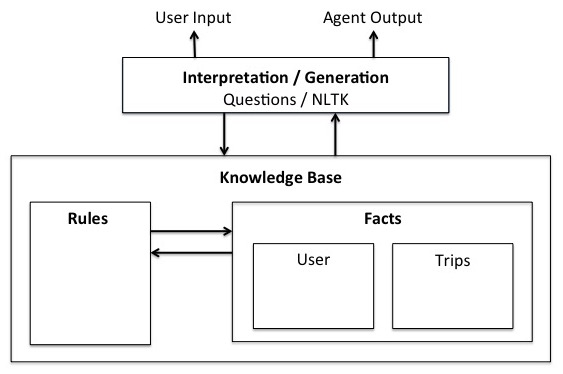
\includegraphics[width=12cm]{architecture.jpg}
\caption{Proposed design for the overall architecture.}
\end{figure}

The agent itself will be written and designed using the
knowledge engine, PyKE, which is a Python module for logic
programming based on the popular PROLOG language.
PyKE provides us with three kinds of knowledge bases,
the Knowledge Fact Base, the Knowledge Rule Base and
the Knowledge Question Base.

The Knowledge Fact Base will contain all the facts we
know about the user, such as; name, previous trips, travel
possessions, the trips themselves (with associated
locations, weather conditions, interesting sites,
attractions, and activities).

The Rule Base will be used to encode how the program
will make connections between the user’s preferences
stored as beliefs and the trips. It will also try to match
the user to other users in its knowledge base to find
trips that similar users have taken and enjoyed and
recommend them to the current user.

The Question Base can be used to store questions to ask
the user to enquire about their preferences. The
structure of this seems a little inflexible though
upon first impression since we aim for a more natural
feeling dialog than pre-coded questions so the usefulness
of this tool for our system is still up for debate.

A different option for realising a natural language
user dialog is employing the Natural Language Toolkit
(NLTK) for python. NLTK provides different modules
for natural language processing such as lexicons,
parsers or text classification that can be used to
map the user input to a number of discourse acts in
order to extract the relevant information and update
the belief system.

\section{References}
%References and such
(1) Marc Cavazza, Cameron Smith, Daniel Charlton, Li Zhang, Markku Turunen, and Jaakko Hakulinen. 2008. A 'companion' ECA with planning and activity modelling. In Proceedings of the 7th international joint conference on Autonomous agents and multiagent systems - Volume 3(AAMAS '08), Vol. 3. International Foundation for Autonomous Agents and Multiagent Systems, Richland, SC, 1281-1284.\\
(2) Ricci, Francesco, et al. "ITR: a case-based travel advisory system." Advances in Case-Based Reasoning. Springer Berlin Heidelberg, 2002. 613-627.\\
(3) Loper, Edward, and Steven Bird. "NLTK: The natural language toolkit." Proceedings of the ACL-02 Workshop on Effective tools and methodologies for teaching natural language processing and computational linguistics-Volume 1. Association for Computational Linguistics, 2002.

\end{document}
